\section{Simulating and recording scientific data}\label{sec:mat}
History about synthesis, screening, characterization, discovery and re-discovery (retrieval)

%------------------------------------------------------------------------------
\subsection{Cryo-EM}\label{subsec:cryo}
chao/joao
64 by 64 projection images of TFIID along 9 viewing angles with random perturbation, noise free);

\begin{table}[]
\centering
\caption{My caption}
\label{my-label}
\begin{tabular}{|c|c|c|}
 $\Psi\downarrow_i$    & $\Theta\downarrow_i$       & $\phi\downarrow_i$       \\
0.00 & 0.0000 & 0.0000 \\
0.00 & 45.000 & 0.0000 \\
0.00 & 45.000 & 89.975 \\
0.00 & 45.000 & 179.95 \\
0.00 & 45.000 & 269.92 \\
0.00 & 90.000 & 0.0000 \\
0.00 & 90.000 & 59.983 \\
0.00 & 90.000 & 119.97 \\
0.00 & 90.000 & 178.95
\end{tabular}
\end{table}

\textbf{Classifying 9 views:}
Training images generated from a 3D density map of a transcription factor-II

\textbf{Testing}
100 projection images generated from Euler angles
 chosen randomly from 1 to 9
,  generated randomly (uniform distribution) with
Result: 100\% success rate





9 views (evenly spaced on a sphere)
1000 simulated projection images
Projection Euler angles:

 chosen randomly from 1 to 9
,  generated randomly (uniform distribution) with

\begin{figure*}[!t]
\centering
\subfloat[Experimental molecule projections]{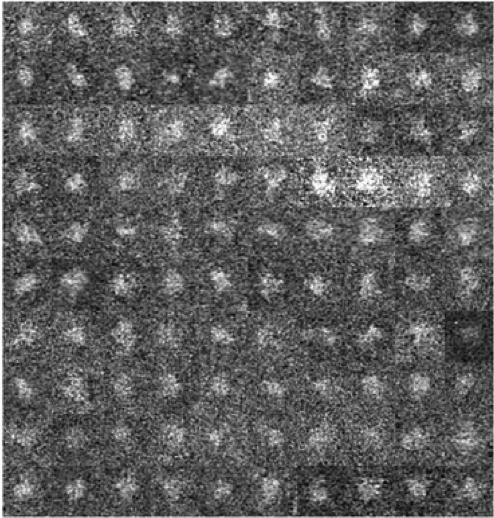
\includegraphics[width=.314\linewidth]{img/cryoem3a.png}
\label{fig_first_case}}
\hfil
\subfloat[Detected particle projections]{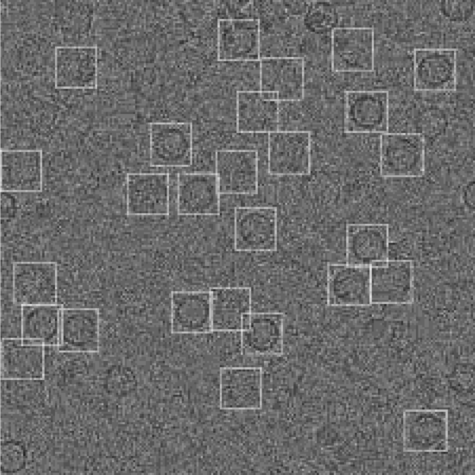
\includegraphics[width=.33\linewidth]{img/cryoem3b.png}
\label{fig_second_case}}
\subfloat[Simulated molecule projections]{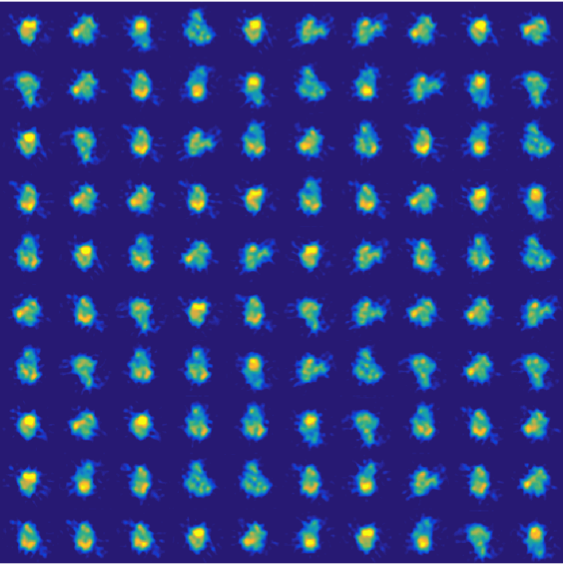
\includegraphics[width=.33\linewidth]{img/cryoem3c.png}
\label{fig_second_case}}
\caption{LDRD case.}
\label{fig:ldrd}
\end{figure*}

\begin{figure*}[!t]
\centering
\subfloat[TFIIDM molecule]{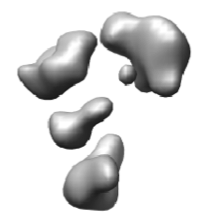
\includegraphics[width=.32\linewidth]{img/cryoem1.png}
\label{fig_first_case}}
\hfil
\subfloat[Projections model]{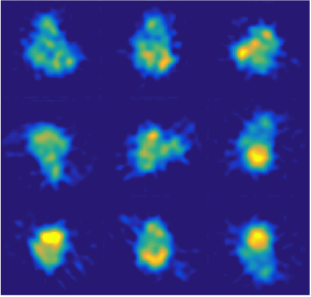
\includegraphics[width=.32\linewidth]{img/cryoem1b.png}
\label{fig_second_case}}
\subfloat[Compact model]{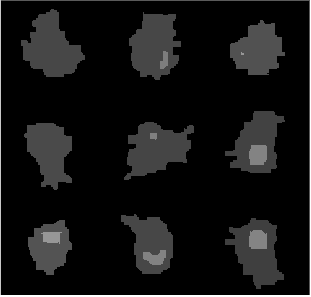
\includegraphics[width=.32\linewidth]{img/cryoem1c.png}
\label{fig_second_case}}
\caption{LDRD case.}
\label{fig:ldrd}
\end{figure*}


%------------------------------------------------------------------------------
\subsection{X-ray diffraction}\label{subsec:diffraction} %LDRD Bragg peaks
92\% success rate for good images
96\% success rate for bad images
Sufficiently good to distinguish good images from bad images
%92% success rate on images with Bragg peaks
%96% success rate on images with few Bragg peaks

\begin{figure}[!t]
\centering
\subfloat[Hit]{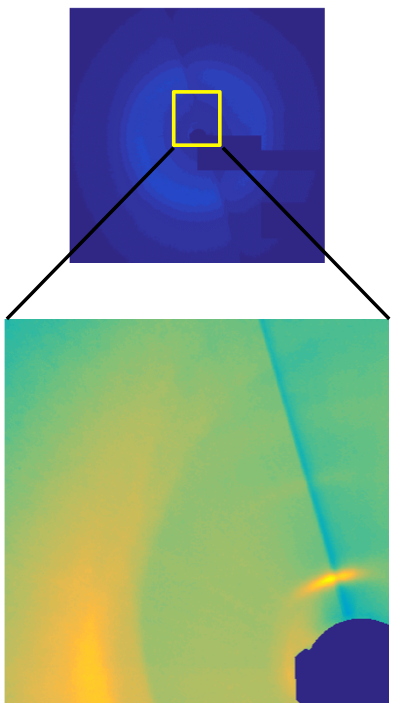
\includegraphics[width=.33\linewidth]{img/bragg1.png}
\label{fig_first_case}}
\hfil
\subfloat[Miss]{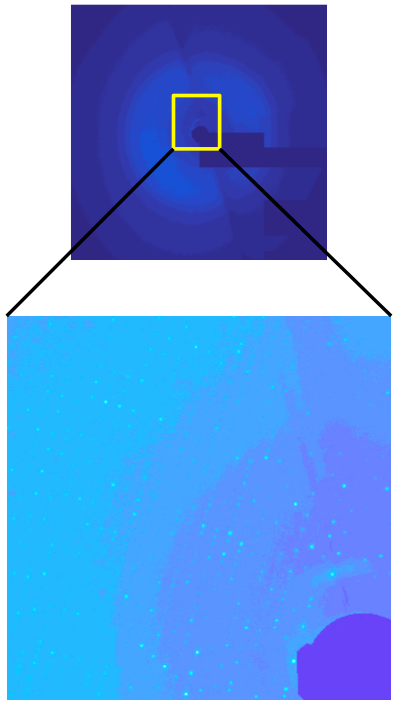
\includegraphics[width=.33\linewidth]{img/bragg2.png}
\label{fig_second_case}}
\caption{LDRD case - bragg peaks.}
\label{fig:ldrd}
\end{figure}

\begin{figure}[!t]
\centering
\subfloat[False negative]{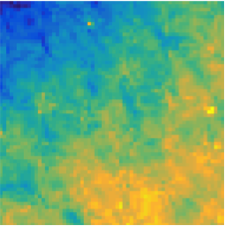
\includegraphics[width=.33\linewidth]{img/xdiffraction_falsenegative.png}
\label{fig_first_case}}
\hfil
\subfloat[False positive]{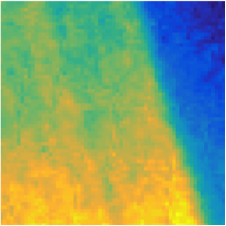
\includegraphics[width=.33\linewidth]{img/xdiffraction_falsepositive.png}
\label{fig_second_case}}
\caption{LDRD case - bragg peaks.}
\label{fig:ldrd}
\end{figure}



%------------------------------------------------------------------------------
\subsection{X-ray scattering}\label{subsec:scattering}
We propose a supervised classification approach to identify the crystal lattice types from a Grazing
Incidence Small Angle X-ray Scattering (GISAXS) image. GISAXS is an important reciprocal-space imaging
modality which provides statistical information about a sample in 3-D. GISAXS is widely used for
studying thin films that play a vital role as building blocks for the next generation of renewable
energy technology. One challenge in GISAXS imaging is to accurately infer the crystal lattice
corresponding to the sample from a single 2-D diffraction/scatter pattern.

As a first step towards understanding crystal configurations, we use a simulation package termed
HiPGISAXS [1], to generate a large collection of sample images from each class of possible crystal
structures and test the algorithm performance under multiple simulated test images. Inspired by the
recent success of deep-learning approaches for natural image classification, we use a Convolutional
Neural Network (CNN) [2] method to carry out the classification.

We address the problem of classifying GISAXS patterns from 7 different crystal lattices (classes). We
generated 1,000 images with dimensions of 100X100 pixels for each class by varying the lattice
parameters as input to a 4 layer CNN to train a classifier. The architecture of this network is
adapted from the MNIST classifier used by MatConvNet. We tested the performance of the classifier on
multiple data sets, including samples corrupted with realistic noise levels. We obtained an accuracy
that ranged from 82.6\% to 92.29\% depending on the parameters of each test case which we believe is
an encouraging result for further extending the use of CNNs for GISAXS as well as other synchrotron
based scientific experiments.

\begin{table}[]
\centering
\caption{My caption}
\label{my-label}
\begin{tabular}{llll}
Method & dataset1 & dataset2 & noisyDataset \\
CNN    & 92.29    & 82.60    & 91.57        \\
HOG    & 92.00    & 79.88    & 79.57        \\
       &          &          &
\end{tabular}
\end{table}

%------------------------------------------------------------------------------
\subsection{X-ray attenuation}\label{subsec:microct}

\begin{figure*}[h]
\centering
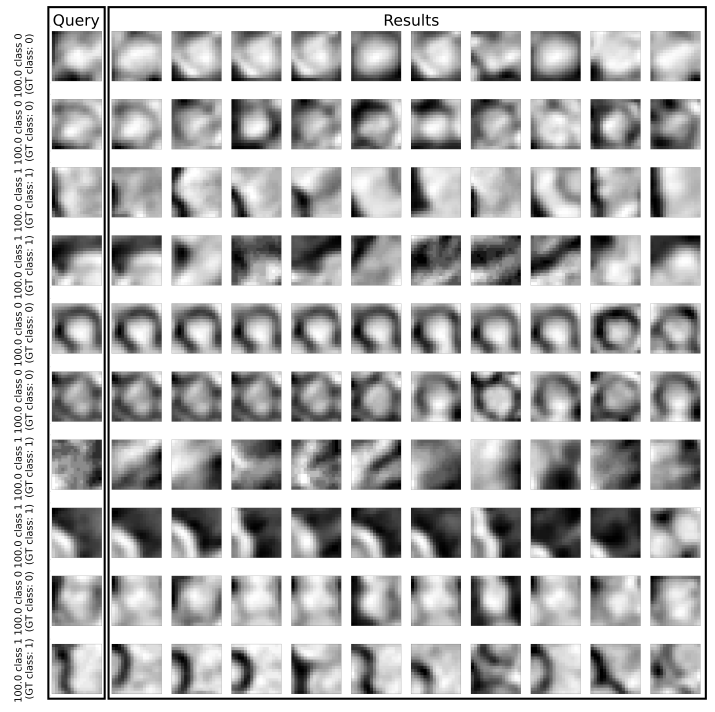
\includegraphics[width=\linewidth]{img/fiberResult.png}
\caption{Fiber result.}
\label{fig:fiberResult}
\end{figure*}
